\begin{frame}
	\frametitle{Corollaries}
	\begin{corollary}
		The results we have given for \(\kappa\)-node MEMs, \(\kappa\)-node MEMs spanning
		exactly \(L\) nodes and EFGs hold when \(Q[1..m]\) is replaced by a set of
		queries of total length \(m\).
	\end{corollary}
	\onslide<2>\begin{corollary}
		The algorithms we have given before (including the corollary above) can be modified
		to report only MEMs that occur in text \(T\) formed by concatenating the rows (ignoring
		gaps and adding separator symbols) of the input MSA of the indexable EFG.
	\end{corollary}
	This can be done in additional \(O(|T | + r \log r)\) time and \(O(r \log n)\) bits of space,
	and with multiplicative factor \(O(\log \log n)\) added to the running times
	of the respective algorithms, where \(r\) is the number of equal-letter runs in the BWT of \(T\).
\end{frame}

\begin{frame}
	\frametitle{Experimental results}
	\framesubtitle{Number of MEMs with different indices and varying number of covid19 strains}
	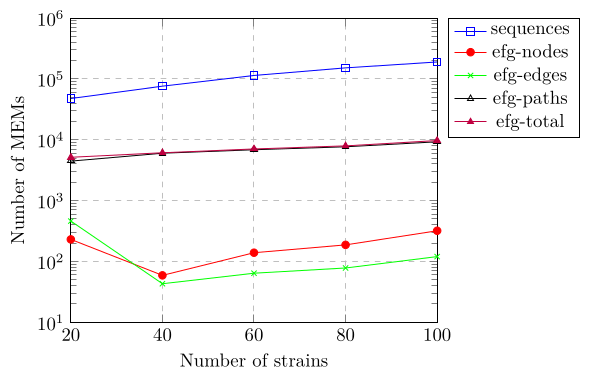
\includegraphics[scale=0.5]{images/number-of-mems.png}
\end{frame}

\begin{frame}
	\frametitle{Experimental results}
	\framesubtitle{Number of BWT runs with different indexes and varying number of covid19 strains}
	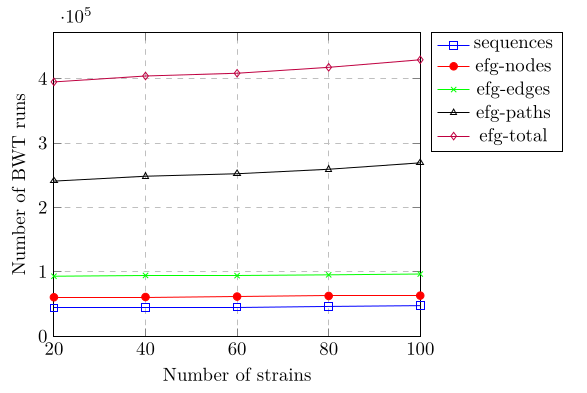
\includegraphics[scale=0.5]{images/number-of-bwt-runs.png}
\end{frame}